
% --- 1. Introduction ---
The project is divided into three core streams:
\begin{itemize}
    \item \textbf{Locomotion:} Developing capability of the robot to traverse rough terrain
    \item \textbf{Perception:} Developing capability of the robot to sense its environment and take decisions, e.g. with regards to posture adaptation
    \item \textbf{Simulation:} Developing an accurate virtual environment to safely implement, test, and iterate over the locomotion and perception strategies before hardware deployment
\end{itemize}

% --- 2. Functional Requirements ---
\section{Functional Requirements}

\subsection{Simulation}
\begin{itemize}
    \item The simulation system must allow for randomly generating environments
    \item The simulated environments must have rough terrain
    \item The simulated environments must have narrow passages, areas with low ceilings, and protrusions from the ground to test posture adaptation
    \item The generation process must include parameters for adjusting roughness in terrain, ground friction, range of width and height of passages, and range of size of protrusions
    \item The simulation system must support physics
    \item The T-Hex robot must be simulated with user-defined mass properties
\end{itemize}

\subsection{Perception}
\begin{itemize}
    \item The robot must be integrated with a camera to be attached on the robot in simulation
    \item The robot must be able to build a map of the immediate environment in simulation, i.e., what is directly ahead of the robot 
    \item The robot must be able to use a map of the immediate environment in simulation to make decisions to switch to a narrower posture to pass through thin passages, a shorter posture to pass under low ceilings, or a posture with higher body clearance to pass over protrusions
\end{itemize}

\subsection{Locomotion}
\begin{itemize}
    \item The robot, in both simulation and hardware, should be able to walk on flat and rough terrain
    \item The robot, in both simulation and hardware, should be able to adapt its posture in both flat and rough terrains
    \item The robot, in both simulation and hardware, must be teleoperable - it should take a target position relative to itself as input and execute a straight line trajectory to reach it, adjusting to the terrain and obstacles
\end{itemize}
% \begin{itemize}
%     \item \textbf{Gait Scheduling:}
%         \item The system must implement an open-loop kinematic gait for basic walking and testing.
%         \item The system must implement a dynamic gait scheduler that determines which legs are in the stance phase and which are in the swing phase at any given time.
%     \item \textbf{Trajectory Generation:}
%         \item The system must compute a desired Center of Mass (CoM) trajectory based on operator commands and the current gait schedule.
%         \item The system must generate smooth swing leg trajectories (e.g., using splines) to move a leg from its current position to a desired foothold.
%     \item \textbf{Dynamic Control:}
%         \item The system must plan optimal footholds for swing legs based on the robot's velocity and terrain data (e.g., using Raibert's heuristic).
%         \item The system must calculate the optimal Ground Reaction Forces (GRFs) for all stance legs to maintain balance and follow the desired CoM trajectory. This shall be achieved via a model-based controller (e.g., Balance Controller with QP or Convex MPC).
%         \item The system must translate desired forces (for stance legs) and desired positions (for swing legs) into final joint torque commands using a Joint PD Controller.
%     \item \textbf{Posture Adaptation:}
%         \item The system must use perception data to autonomously adapt the robot's body posture (height, roll, pitch).
%         \item The system must be able to lower its posture to navigate under low overhangs and narrow its posture to pass through thin gaps.
    
%     \item The system must estimate the robot's Center of Mass (CoM) state; that is, its position, velocity, and orientation.
%     \item The system must be able to detect whether a leg is in contact with the ground (stance) or in the air (swing).
% \end{itemize}

% --- 3. Non-Functional Requirements ---
\section{Non-Functional Requirements}

\begin{itemize}
    \item The robot should be able to walk in terrains with local vertical step size up to 8cm
    \item The robot should be able to walk in terrains with local slope up to 15 degrees
    \item The robot should be able to pass through passages as narrow as 38cm in simulation
    \item The robot should be able to pass through areas with ceilings as low as 16cm in simulation
    \item The robot should be able to pass over protrusions of up to 6cm in simulation
    \item The robot should be able to walk in terrains with friction coefficient of 0.5-0.7
    \item The robot should be able to walk in terrains with sand, ash, and pebbles as big as 1cm
    \item There must be at least three ``postures'' that the robot should be able to move in: a shorter posture, a regular posture, and a posture with higher body clearance in simulation
    \item For data integrity purposes, there must be a Docker image containing everything necessary to run the simulation of the robot in randomly generated environments
    \item The entire codebase must be well-commented with citations included in either the README or as comments in the file themselves for code that is taken or adopted from someplace else
    \item The entire codebase must be well-structured and maintained with complete version control on GitHub to allow for backups in case of catastrophe
    \item Documents detailing the robot's hardware architecture and its locomotion and perception strategy must be prepared
\end{itemize}

% \subsection{Performance}
% \begin{itemize}
%     \item The system must generate the multi-elevation map and pass it to the path planner at a frequency of 1-4 Hz.

%     \item The mapping algorithms must be fast enough to avoid bottlenecks in the perception pipeline.

%     \item The height information must be granular enough for the robot to navigate terrain and obstacles.

%     \item The system must cluster sensor data into "floor" and "ceiling" elevations with sufficient accuracy.

%     \item The perception system must account for drift in odometry.

%     \item The system map must maintain reliability of data and discard outdated information over time.

%     \item The system must account for sensor bias, variance, and noise/

%     \item The system must be able to function in a real environment imitating a lava tube.

%     \item The dynamic balance controller must execute in real-time to ensure stability. The low-level Joint PD Control loop must run at a frequency of at least 500 Hz.
%     \item The robot must draw a stable current to operate. The system must manage power, noting that standing alone draws 4A. The final design should explore battery operation.
% \end{itemize}

% % \subsection{Security}
% % \begin{itemize}
% %     \item \textbf{Control Link:} Any wireless communication between the operator GUI and the robot must be encrypted to prevent unauthorized commands.
% %     \item \textbf{Onboard System:} The Raspberry Pi or other onboard computer must be hardened (e.g., disabled default passwords, firewall) to prevent unauthorized network access.
% % \end{itemize}

% \subsection{Reliability}
% \begin{itemize}
%     \item The system must be robust against general hardware failures. 
%     \item The control software must, given significant unexpected contact or sensor failures, enter a safe state immediately without further damage.
%     \item The RPi or SSC32 should not crash unexpectedly.
% \end{itemize}

% \subsection{Usability}
% \begin{itemize}
%     \item The simulation GUI must be easy enough for a typical robotics undergraduate to control the robot.
%     \item The simulation environment and its parameters must be easy to configure.
% \end{itemize}

% \subsection{Data Integrity}
% \begin{itemize}
%     \item Sensor data must be timestamped accurately to ensure proper state estimation.
%     \item The state estimator must validate inputs from the sensor to minimize robot state error.
% \end{itemize}

% \subsection{Backup}
% \begin{itemize}
%     \item A remote repository must be set up for version control of all code.
%     \item Logs must be kept for metrics obtained from simulation and physical trials.
% \end{itemize}

\section{Use Cases}
We have only one user: the Operator. For that, the following use cases are defined:
\begin{itemize}
    \item \textbf{Commands:} The operator gives position commands relative to the robot
    \item \textbf{Adjust simulation parameters:} The operator is able to adjust the parameters of the simulation environment
    \item \textbf{Generate simulation environment:} The operator is able to generate simulation environments
    \item \textbf{Pick and place simulated robot:} The operator is able to move the simulated robot by picking it up and placing it at the desired position
\end{itemize}

\begin{figure}[H]
    \centering
    % --- NOTE: You must create this image file (use_case_diagram.png) ---
    % --- You can use a tool like Lucidchart or diagrams.net      ---
    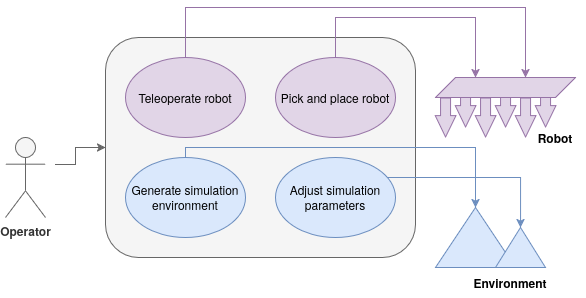
\includegraphics[width=0.6\textwidth]{UseCase.png}
    \caption{Use Case Diagram for the Legged Robot System.}
    \label{fig:use_case}
\end{figure}

\section{Block Diagrams}



\subsection{Perception}


In simulation, the camera takes in the environment and processes it as RGB-D data. It also possesses the IMU data which will tell about the robot's state. Both of these are used to create an elevation map for the robot to not only know where it is in space, but also how to navigate its environment as well as obstacles. There are converted to a signed distance field; that is, a field determining where is safe for the robot to proceed without collision; which lead to vertical and lateral clearance that serve as the basis for posture adaptation. This outputs a posture adaptation signal determining a desired height for the robot, which is sent to the locomotion algorithm. (The width is inferred from the height as described later.)


\begin{figure}[H]
    \centering
    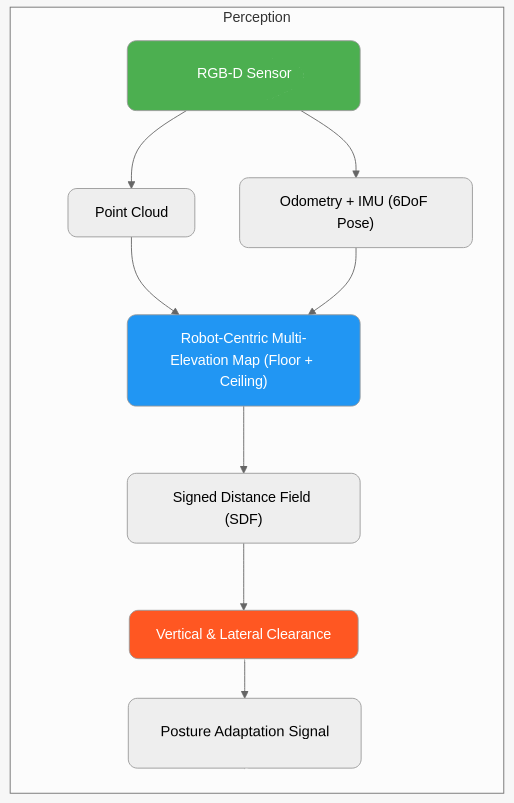
\includegraphics[width=0.5\linewidth]{Perception Diagram.png}
    \caption{Perception Diagram for the Legged Robot System.}
    \label{fig:perception}
\end{figure}

\subsection{Locomotion}

The first of the three locomotion algorithms we have covered is the simplest: the kinematic gait. This operates on a gait schedule, which defines stance and swing legs with their own trajectories. Once generated, the trajectories are tracked before sent as motor commands.

\begin{figure}[H]
    \centering
    % --- NOTE: You must create this image file (use_case_diagram.png) ---
    % --- You can use a tool like Lucidchart or diagrams.net      ---
    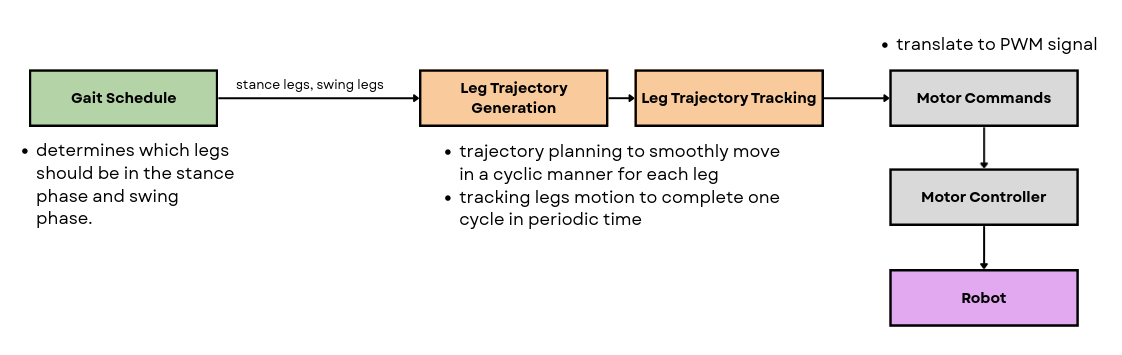
\includegraphics[width=1.0\textwidth]{Locomotion0.png}
    \caption{Kinematic Locomotion Diagram for the Legged Robot System.}
    \label{fig:kinematic_locomotion}
\end{figure}


The next diagram represents the general locomotion architecture that is observed in literature. Based on user commands and the persistent gait schedule, a trajectory for the robot's center of mass is planned, which is used to solve for the forces exerted by the legs in stance (i.e., in contact with the ground) and to generate the trajectories to be generated by the legs in swing. These forces and desired positions are converted into motor commands that are sent to some motor controller and then to the motors. The robot's states (joint positions, roll, pitch, yaw) are incorporated at different steps to ensure robustness.


\begin{figure}[h!]
    \centering
    % --- NOTE: You must create this image file (use_case_diagram.png) ---
    % --- You can use a tool like Lucidchart or diagrams.net      ---
    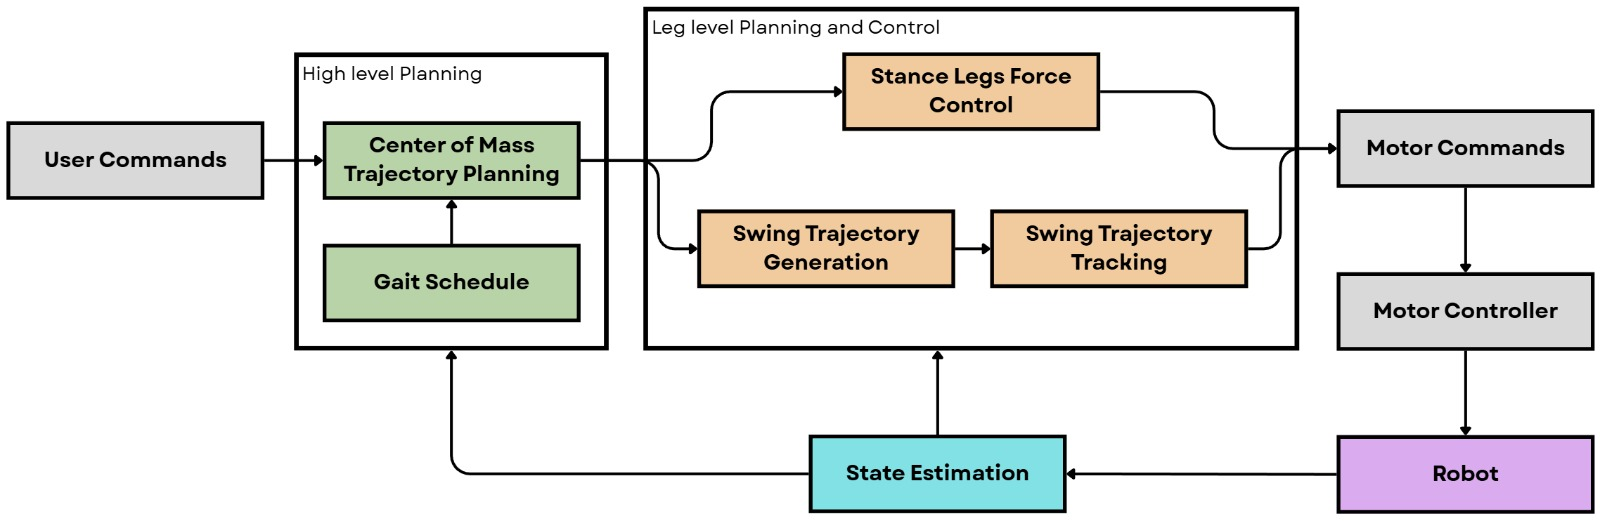
\includegraphics[width=1.0\textwidth]{Locomotion Diagram.png}
    \caption{Dynamic Locomotion Diagram for the Legged Robot System.}
    \label{fig:dynamic_locomotion}
\end{figure}

A third and significant locomotion architecture is that of reinforcement learning (RL). In this case, the policy network starts with user commands and passes its predicted movements as motor commands. Similarly to control, the state estimation segment sends feedback to the network, which adjusts itself accordingly and repeats the cycle. In our case, this particular paradigm's flavor is mixed with a deep learning network, thus being deep reinforcement learning (DRL).

\begin{figure}[h!]
    \centering
    % --- NOTE: You must create this image file (use_case_diagram.png) ---
    % --- You can use a tool like Lucidchart or diagrams.net      ---
    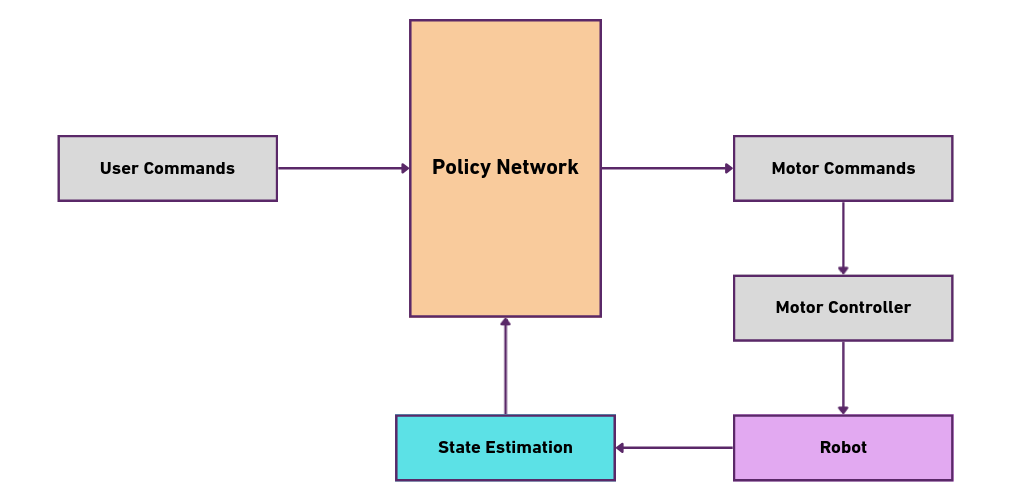
\includegraphics[width=1.0\textwidth]{Locomotion2.png}
    \caption{DRL Locomotion Diagram for the Legged Robot System.}
    \label{fig:drl_locomotion}
\end{figure}


\subsection{Hardware}

\begin{figure}[h!]
    \centering
    % --- NOTE: You must create this image file (use_case_diagram.png) ---
    % --- You can use a tool like Lucidchart or diagrams.net      ---
    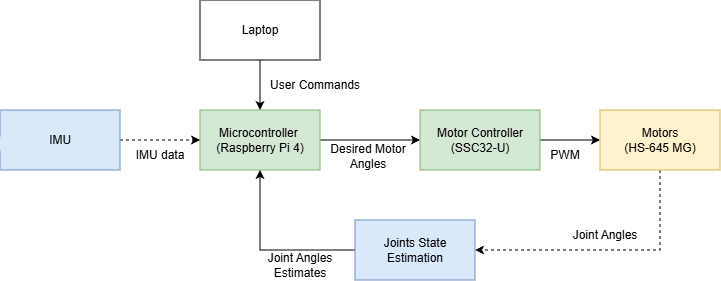
\includegraphics[width=1.0\textwidth]{Hardware Diagram.png}
    \caption{Hardware Diagram for the Legged Robot System. Lines indicate the flow of data, with dotted lines indicating the robot states or world states being observed}
    \label{fig:hardware}
\end{figure}

Our system contains hardware modules depicted in the diagram above. The microcontroller receives user commands from the user's laptop, IMU data from the IMU, and estimates of the robot legs' joint angles from some state estimation method (e.g., motor encoders or motion capture cameras). The microcontroller runs the locomotion algorithms and outputs desired motor angles to the separate motor controller. The motor controller then generates pulse width modulation (PWM) signals that are received by the motors.
